\chapter{Results} \label{study_results}

This Chapter describes all the results gathered throughout the study in a per RQ basis. This approach increase the traceability of the findings within the report as suggested by Runeson et al. \cite{case_study_software_engineering} (Item 20 in Appendix \ref{checklist_for_case_studies}).

Furthermore, to further increase the traceability of concepts from Research questions to results these are presented in a per-research question base with distinction between quantitative and qualitative data.

As a final note, due to confidentiality issues it was not possible to report the raw data. For this reason, as briefly explained in the previous Chapter, all the sensitive information has been eliminated.

\section{Research Question 1}

Results for this Research Question are mostly quantitative. However, some of the codes generated during coding procedures are tied to the issue this particular question addresses.

\subsection{Qualitative Results}
    The thematic analysis reported used to extrapolate information from qualitative data yielded five codes that can be tied to Research Question 1. These items are reported in Table \ref{tab:themes_rq1}. Furthermore, Fig. \ref{fig:sources_of_codes_rq1} shows through which data and the quantity of mentions each of the listed codes received.
    
\begin{table}
\renewcommand{\arraystretch}{1.5}
\centering
\begin{tabular}{ c p{4.3cm} p{4.6cm}}
    
    \hline       
    {\large Global Theme} & {\large Organizing Theme} & {\large Codes}\\
    \hline
    
    \multirow{4}{*}{\parbox[t]{4.3cm}{
        Source code bad habits that also arise in Test code}
    } & \multirow{2}{*}{\parbox[t]{4.3cm}{Modularity related issues}}
        & Over complex functions \\
        & & DRY violations\\ 
        & & God functions\\ \cline{2-3}
        
    & \multirow{2}{*}{\parbox[t]{4.6cm}{Line related issues}}
        & Over complex statements \\
        & & Arity problems \\
    \hline
\end{tabular}
\caption{Themes and codes related to RQ1 extrapolated from qualitative sources}
\label{tab:themes_rq1}
\end{table}

\begin{figure}[!Htb]
    \centering
    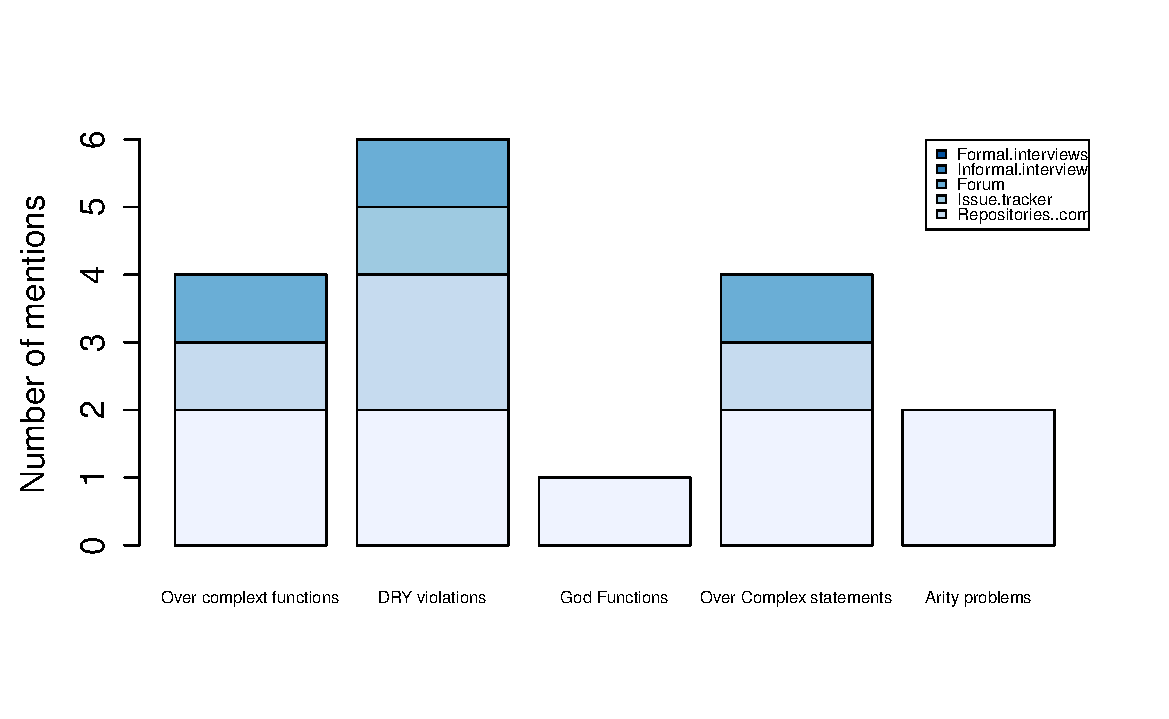
\includegraphics[width=\textwidth,keepaspectratio]{figure/results/rq1/sources.eps}
    \caption{Codes with relatives Data sources}
    \label{fig:rq1_sources}
\end{figure}

\subsection{Quantitative Results}

    As highlighted in the Related Works (section \ref{sec:related_work}), quantitative data has been extracted through static analysis of the code base. However, given the exploratory nature of this study and resources' scarcity, only few metrics have been extracted and analyzed at this stage. Figures \ref{fig:project_a_avg_complexity},\ref{fig:project_b_avg_complexity},\ref{fig:project_c_avg_complexity}, and \ref{fig:project_d_avg_complexity} display results generated by the process previously described in section \ref{sec:analysis_of_the_repos}.
    
    \todo{Fix legends in charts}
    
\begin{figure}[!Htb]
    \centering
    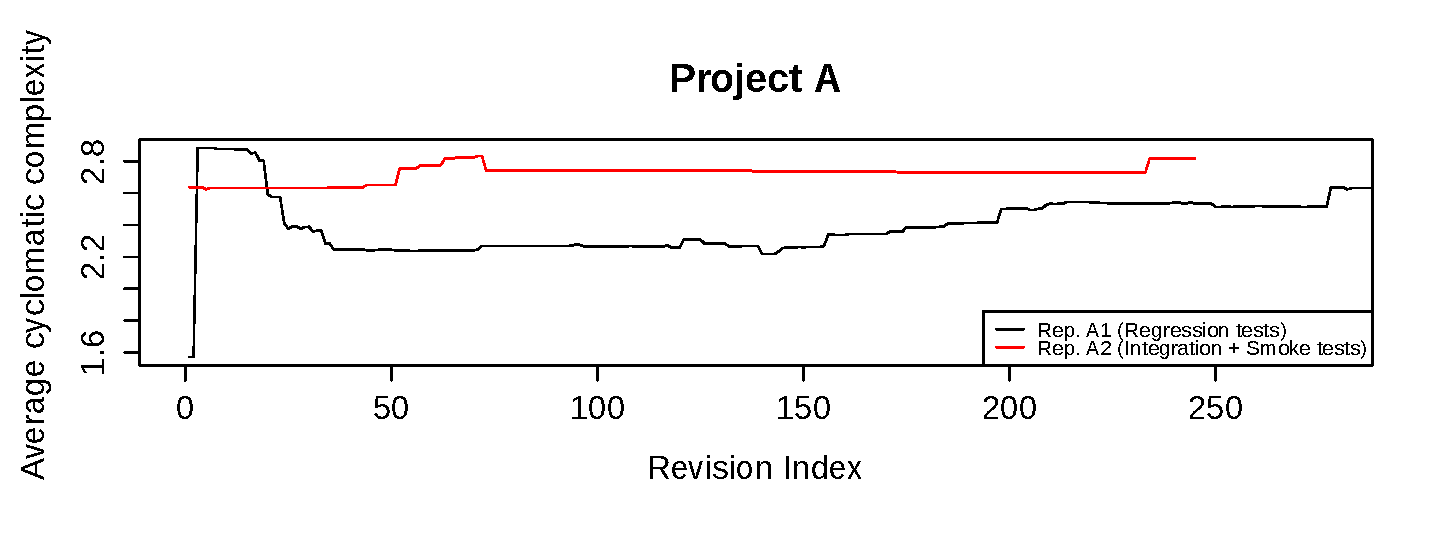
\includegraphics[width=\textwidth,keepaspectratio]{figure/results/rq1/project_a_avg_complexity.eps}
    \caption{Project A average cyclomatic complexity over time}
    \label{fig:project_a_avg_complexity}
\end{figure}

\begin{figure}[!Htb]
    \centering
    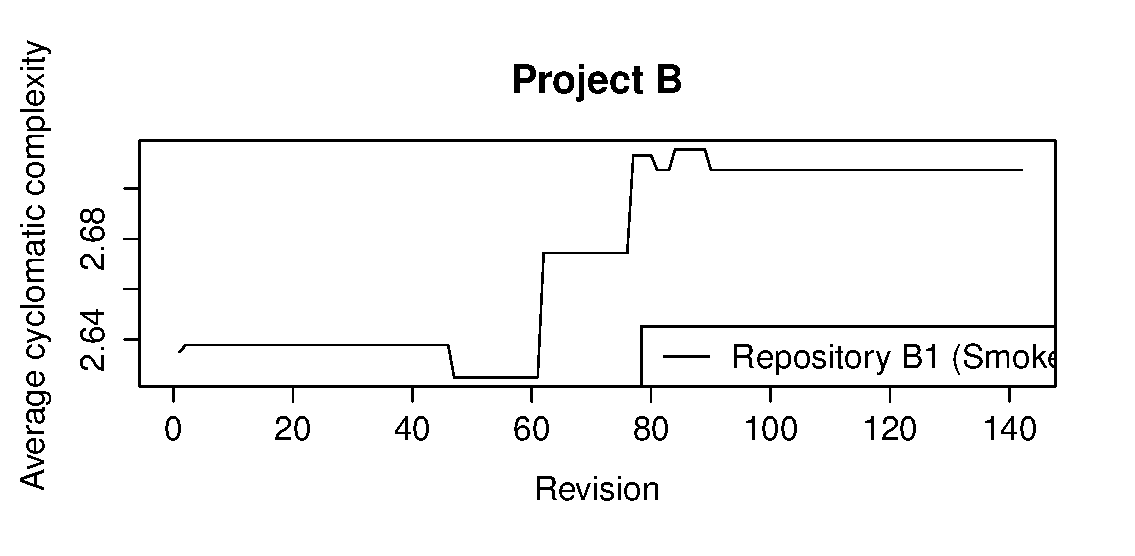
\includegraphics[width=\textwidth,keepaspectratio]{figure/results/rq1/project_b_avg_complexity.eps}
    \caption{Project B average cyclomatic complexity over time}
    \label{fig:project_b_avg_complexity}
\end{figure}

\begin{figure}[!Htb]
    \centering
    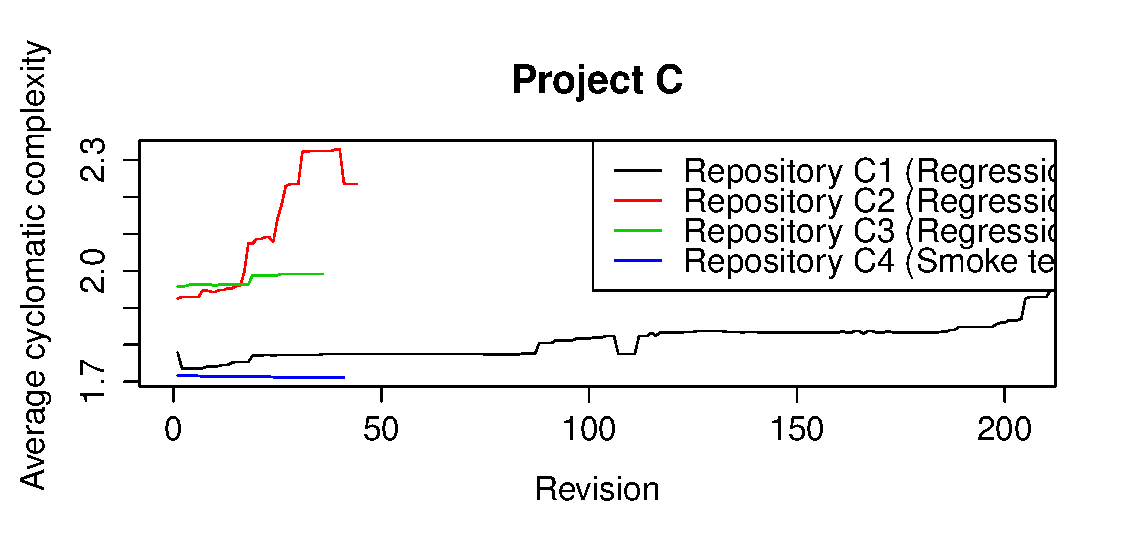
\includegraphics[width=\textwidth,keepaspectratio]{figure/results/rq1/project_c_avg_complexity.eps}
    \caption{Project C average cyclomatic complexity over time}
    \label{fig:project_c_avg_complexity}
\end{figure}

\begin{figure}[!Htb]
    \centering
    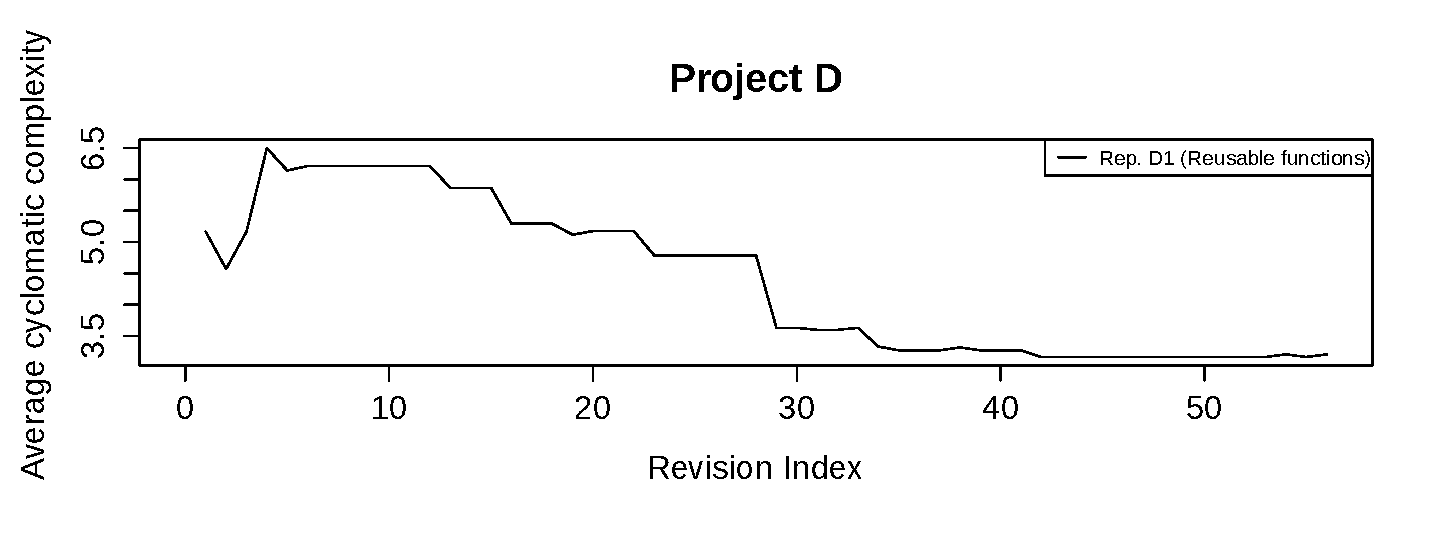
\includegraphics[width=\textwidth,keepaspectratio]{figure/results/rq1/project_d_avg_complexity.eps}
    \caption{Project D average cyclomatic complexity over time}
    \label{fig:project_d_avg_complexity}
\end{figure}




\section{Research Question 2}

The scope of User Interface tests is to validate the state of the User Interface after a predefined series of actions occurred. However, this entails a different use for the constructs compared to conventional source code and possibly new ones specific for these use cases. For this reason the second RQ will inspect these unique items.

However, keeping into account the differences between property based testing and image recognition testing is important. The former uses property or meta-properties of UI components to identify them and simulate user events over them. The latter, instead, uses image recognition algorithms to identify such widgets. This different identification method imposes different approached when creating the test suite that are analyzed separately in the following sections, presenting both quantitative and qualitative results.

\subsection{Qualitative Data}
  As for Research Question 1, thematic analysis has been used to generate a list of recurring codes that can be attributed to user interface specific testware. Precisely, the inquiry resulted in a total of seven codes shown in Table \ref{tab:themes_rq2}.
  
\begin{table}
\renewcommand{\arraystretch}{1.5}
\centering
\begin{tabular}{ c p{4.3cm} p{4.6cm}}
    
    \hline       
    {\large Global Theme} & {\large Organizing Theme} & {\large Codes}\\
    \hline
    
    \multirow{7}{*}{\parbox[b]{4.3cm}{
        User interface testware specific issues
    }
    } & \multirow{4}{*}{\parbox[c]{4.3cm}{Image recognition problems}}
        & Too sensitive \\
        & & False positive and negative results\\
        & & Not reusable\\ 
        & & Not suitable for responsive environments (e.g. web applications)\\ \cline{2-3}
        
    & Property based problems & Impossible to foresee when it will break\\ \cline{2-3}
        
    & Coordinated based problems  & Too fragile\\ \cline{2-3}
        
    & UFT specific problems & Based on binary files\\
        
    \hline
\end{tabular}
\caption{Themes and codes related to RQ1 extrapolated from qualitative sources}
\label{tab:themes_rq2}
\end{table}


\section{Research Question 3}

Finally, the purpose of this RQ is to complete the description of the TD items identified by RQ 1 and RQ 2. Once again, qualitative and quantitative data has been treated separately.

\subsection{Qualitative Data}
    

\subsection{Quantitative Data}
    

